\documentclass[10pt,notes,compress,aspectratio=169]{beamer}
\usepackage[brazil]{babel}  
\usepackage[utf8]{inputenc}
\usepackage[T1]{fontenc}

\usefonttheme[onlymath]{serif}
\usepackage{beamerthemesplit}
\usetheme{Antibes}

\beamersetuncovermixins{\opaqueness<1->{25}}{\opaqueness<2->{15}}
\setbeamertemplate{itemize items}[triangle]
\setbeamertemplate{enumerate item}{\insertenumlabel)}
\setbeamertemplate{enumerate subitem}{\insertenumlabel-\insertsubenumlabel)}
\setbeamertemplate{caption}[numbered]
\setbeamertemplate{mini frames}{}
\setbeamertemplate{navigation symbols}{}
\setbeamerfont{block title}{size=\scriptsize}
\setbeamerfont{frametitle}{size=\small}
\beamertemplatenavigationsymbolsempty

%%%%%%%%%%%%%%%%%%%%%
% defining frametitle
\setbeamertemplate{frametitle}{%
    \nointerlineskip%
    \begin{beamercolorbox}[wd=\paperwidth,ht=2.5ex,dp=1.0ex]{frametitle}
        \hspace*{2.5ex}\insertframetitle%
    \end{beamercolorbox}%
}
%%%%%%%%%%%%%%%%%%%%%

\newcommand{\hrefcolor}[2]{\textcolor{BlueGreen}{\href{#1}{#2}}}

% Rotating Objects and Captions
\usepackage{hvfloat}

% bibliography stuff
\usepackage{natbib}
\usepackage{bibentry}
\nobibliography*

\usepackage[brazilian]{cleveref}
\crefname{lstlisting}{lista}{listas}
\Crefname{lstlisting}{Lista}{Listas}

% equation stuff
\usepackage{nicefrac}
\usepackage{cancel}

% table diagonal box
\usepackage{diagbox}
\usepackage{makecell}

% tables
\usepackage{booktabs}

% BEGIN - listings - code in LaTeX
\usepackage{listings}
\renewcommand\lstlistingname{Lista}
\lstset{
  language=octave,
  breaklines=true,
  postbreak=\mbox{$\hookrightarrow$\space},
  basicstyle=\linespread{1}\small\ttfamily,
  %numbers=left,
  numbers=none,
  %frame=lines,
  xleftmargin=0.5cm,
  frame=none,
  framexleftmargin=0.5em,
  framexrightmargin=0.5em,
  %backgroundcolor=\color{light-gray},
  showstringspaces=false,
  upquote=true,
  commentstyle=\color{gray},
  %morecomment=[f][\color{gray}][28]{\#},
  morecomment=[l]{\#\#},
  literate=%
           {á}{{\'a}}1
           {í}{{\'i}}1
           {é}{{\'e}}1
           {ú}{{\'u}}1
           {ó}{{\'o}}1
           {à}{{\`a}}1
           {ã}{{\~a}}1
           {õ}{{\~o}}1
           {â}{{\^a}}1
           {ê}{{\^e}}1
           {ô}{{\^o}}1
           {ç}{{\c{c}}}1
           {Á}{{\'A}}1
           {Í}{{\'I}}1
           {É}{{\'E}}1
           {Ú}{{\'U}}1
           {Ó}{{\'O}}1
           {À}{{\`A}}1
           {Ã}{{\~A}}1
           {Õ}{{\~O}}1
           {Â}{{\^A}}1
           {Ê}{{\^E}}1
           {Ô}{{\^O}}1
           {Ç}{{\c{C}}}1
}
% END - listings

%\usepackage{amsthm}
%\newtheorem{theorem}{Theorem}
%\newtheorem{corollary}{Corollary}
%\newtheorem{lemma}{Lemma}
\newtheorem{proposition}{Proposition}
\newtheorem{axiom}{Axiom}
%\newtheorem{example}{Example}
%\newtheorem{definition}{Definition}
\newtheorem{remark}{Remark}

\usepackage{etoolbox}
\patchcmd{\theorem}{Theorem}{Teorema}{}{}
\patchcmd{\corollary}{Corollary}{Corolário}{}{}
\patchcmd{\lemma}{Lemma}{Lema}{}{}
\patchcmd{\proposition}{Proposition}{Proposição}{}{}
\patchcmd{\axiom}{Axiom}{Axioma}{}{}
\patchcmd{\example}{Example}{Exemplo}{}{}
\patchcmd{\definition}{Definition}{Definição}{}{}
\patchcmd{\remark}{Remark}{Observação}{}{}

%\patchcmd{\theorem}{Theorem}{Teorema}{}{}
%\patchcmd{\corollary}{Corollary}{Corolário}{}{}
%\patchcmd{\lemma}{Lemma}{Lema}{}{}
%\patchcmd{\proposition}{Proposition}{Proposição}{}{}
%\patchcmd{\axiom}{Axiom}{Axioma}{}{}
%\patchcmd{\example}{Example}{Exemplo}{}{}
%\patchcmd{\definition}{Definition}{Definição}{}{}
%\patchcmd{\remark}{Remark}{Observação}{}{}

%\newtheorem{exercise}[theorem]{Exercício}


\newcommand*{\theorembreak}{\usebeamertemplate{theorem end}\framebreak\usebeamertemplate{theorem begin}}
\newcommand*{\proofbreak}{\hfill ...\usebeamertemplate{proof end}\framebreak\usebeamertemplate{proof begin}{\scriptsize\color{gray}continuação...}\\}
\newcommand*{\examplebreak}{\hfill ...\usebeamertemplate{theorem end}\framebreak\usebeamertemplate{theorem begin}{\scriptsize\color{gray}continuação...}\\}
\newcommand*{\exercisebreak}{\hfill ...\usebeamertemplate{theorem end}\framebreak\usebeamertemplate{theorem begin}{\scriptsize\color{gray}continuação...}\\}
\newcommand*{\lemmabreak}{\hfill ...\usebeamertemplate{theorem end}\framebreak\usebeamertemplate{theorem begin}{\scriptsize\color{gray}continuação...}\\}
\newcommand*{\blockbreak}{\hfill ...\usebeamertemplate{block end}\framebreak\usebeamertemplate{block begin}{\scriptsize\color{gray}continuação...}\\}
\newcommand*{\definitionbreak}{\hfill ...\usebeamertemplate{theorem end}\framebreak\usebeamertemplate{theorem begin}{\scriptsize\color{gray}continuação...}\\}

% math symbols

% symbol for independet
\newcommand\independent{\protect\mathpalette{\protect\independenT}{\perp}}
\def\independenT#1#2{\mathrel{\rlap{$#1#2$}\mkern2mu{#1#2}}}
% Real Numbers
\newcommand\RealNumber{{\rm I\!R}}
% Expected value, Variance and Covariance
\newcommand{\E}{\mathrm{E}}
\newcommand{\Var}{\mathrm{Var}}
\newcommand{\Cov}{\mathrm{Cov}}

%%%%%%%%%%%%%%%%%
% math cancel to (down arrow)
\makeatletter
% #1, #2 offset of label   #6 extra width to clear arrowhead
% #3, #4 vector direction  #7 superscript label style
% #5 vector width          #8 superscript label
\def\cantox@vector#1#2#3#4#5#6#7#8{%
  \dimen@.5\p@
  \setbox\z@\vbox{\boxmaxdepth.5\p@
   \hbox{\kern-1.2\p@\kern#1\dimen@$#7{#8}\m@th$}}%
  \ifx\canto@fil\hidewidth  \wd\z@\z@ \else \kern-#6\unitlength \fi
  \ooalign{%
    \canto@fil$\m@th \CancelColor
    \vcenter{\hbox{\dimen@#6\unitlength \kern\dimen@
      \multiply\dimen@#4\divide\dimen@#3 \vrule\@depth\dimen@\@width\z@
      \vector(#3,-#4){#5}%
    }}_{\raise-#2\dimen@\copy\z@\kern-\scriptspace}$%
    \canto@fil \cr
    \hfil \box\@tempboxa \kern\wd\z@ \hfil \cr}}
\def\bcancelto#1#2{\let\canto@vector\cantox@vector\cancelto{#1}{#2}}
\makeatother
%%%%%%%%%%%%%%%%%


%%%%%%%%%%%%%%%%%
% left-right arrow
\makeatletter
\newcommand\xleftrightarrow[2][]{%
  \ext@arrow 9999{\longleftrightarrowfill@}{#1}{#2}}
\newcommand\longleftrightarrowfill@{%
  \arrowfill@\leftarrow\relbar\rightarrow}
\makeatother
%%%%%%%%%%%%%%%%%


%%%%%%%%%%%%%%%%%
% commands to resume enumeration across frames 
\newcounter{sauvegardeenumi}
\newcommand{\asuivre}{\setcounter{sauvegardeenumi}{\theenumi}}
\newcommand{\suite}{\setcounter{enumi}{\thesauvegardeenumi}}
%%%%%%%%%%%%%%%%%

%%%%%%%%%%%%%%%%% underbrase - font size no change
\newcommand*{\KeepStyleUnderBrace}[1]{%
  \mathop{%
    \mathchoice
    {\underbrace{\displaystyle#1}}%
    {\underbrace{\textstyle#1}}%
    {\underbrace{\scriptstyle#1}}%
    {\underbrace{\scriptscriptstyle#1}}%
  }\limits
}
%%%%%%%%%%%%%%%%%

%%%%%%%%%%%%%%%%% math operators
\DeclareMathOperator*{\argmin}{\arg\!\min}
\DeclareMathOperator*{\argmax}{\arg\!\max}
\DeclareMathOperator{\sign}{sign}
\DeclareMathOperator{\Tr}{Tr}
%%%%%%%%%%%%%%%%%


%%%%%%%%%%%%%%%%%
\newenvironment{inlineitemize}{%
 \let\par\relax%
 \def\item{\usebeamertemplate{itemize item}\hspace{1mm}}
 \leavevmode%
}{}

\newenvironment{inlineenumerate}{%
 \let\par\relax%
 \setcounter{enumi}{1}%
 \def\item{\usebeamertemplate{enumerate  item} \stepcounter{enumi}}%
 \leavevmode%
}{%
 \setcounter{enumi}{0}%
}
%%%%%%%%%%%%%%%%%




\title[Processamento de Áudio e Vídeo]{Processamento de Áudio e Vídeo}
\author[Prof. Leonardo Araújo]{Prof. Leonardo Araújo}
\date{}


\begin{document}
\frame{\titlepage}

\frame{\centering 
\includegraphics[width=0.4\textwidth]{images/qrcode-aev.pdf} \\ \url{https://sites.google.com/site/leolca/teaching/multimedia-signal-processing}}

\frame[allowframebreaks]{\begin{footnotesize}\tableofcontents\end{footnotesize}}

% introdução
\section{Introdução}

\begin{frame}%[allowframebreaks]
  \frametitle{Processamento de Áudio e Vídeo}
 
  \begin{itemize}
  \item Compressão
  \item Com/Sem perdas
  \item mp3, jpeg, mpeg, flac, zip, gif, png, etc
  \item sinais de áudio, fala, imagens e vídeo
  \item qualidade, taxa de compressão, custo
  \end{itemize} 

\end{frame}
\note{
  \begin{itemize}
  \item O conceito de compressão surge naturalmente quando estamos lidando com comunicação.
  \item Compressão de dados é o processo de converter dados provenientes de uma fonte em
  outros dados com menor tamanho.
  \item Armazenamento e transmissão (no fundo, ambos são formas de comunicação). 
    \begin{itemize}
    \item linha telefônica analógica
    \item comunicação digital através desta linha telefônica analógica
    \item link de comunicação de rádio entre a sonda espacial Galileu orbitando Júpiter e a Terra
    \item armazenamento e reprodução de áudio ou vídeo (ou dados) em um CD, DVD ou disco rígido
    \item reprodução celular em que a informação sobre as células é contida no DNA
    \end{itemize}
  \end{itemize}
}
\note{
  Métodos de compressão sem perda (alguns são vistos na disciplina Teoria da Informação)
  possuem como limite a entropia. Reconstrução exata da mensagem produzida pela fonte.
  Remover redundância.

  \vspace{2ex}
  Métodos de compressão com perda utilizam-se do fato de que muita informação pode ser 
  perdida sem ser percebida ou aceita-se uma distorção do sinal em prol de uma maior compressão.
}
\note{
\begin{itemize}
\item Áudio, fala, imagens e vídeo são originalmente sinais analógicos.
\item Conversão em sinais digitais: amostragem, quantização, codificação.
\end{itemize}
}
\note{
A qualidade da compressão pode ser uma medida objetiva ou subjetiva.
Na maioria das vezes, iremos realizar medidas objetivas pois realizar
testes subjetivos é muito dispendioso. Podemos escolher medidas objetivas 
que sejam bem correlacionadas com medidas subjetivas.

O custo de compressão e descompressão podem, em geral, serem diferentes.
Descompressão deve ser privilegiada pois é realizada diversas vezes e geralmente
por terminais com menor poder computacional.
}


\begin{frame}%[allowframebreaks]
  \frametitle{Imagem digital}

  \begin{figure}[h]
  \centering
  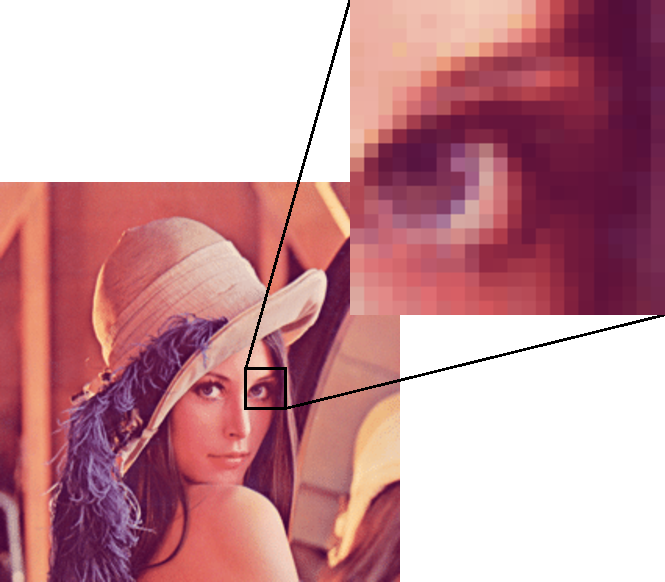
\includegraphics[width=0.5\textwidth]{images/lenaeye.pdf}
  \caption{Lena - detalhe.}\label{fig-lena-detalhe}
  \end{figure}

\end{frame} 

\begin{frame}%[allowframebreaks]
  \frametitle{Espaço necessário para armazenar uma foto}
  \begin{itemize}
  \item câmera 10 Mpixel
  \item 3 bytes por pixel (RGB)
  \item cada foto requer 30 Mbyte
  \item um cartão de memória de 2 Gbytes é capaz de armazenar 66 fotos
  \end{itemize}
\end{frame}

\begin{frame}%[allowframebreaks]
  \frametitle{Espaço necessário para armazenar um vídeo}
  \begin{itemize}
  \item 480 x 720, 30 fps
  \item 345.600 pixels por frame
  \item RGB 3 bytes por pixel
  \item 1.036.800 byte, aprox. 1 Mbyte por frame
  \item 30 frames requerem 31.104.000 bytes, aprox. 31 Mbyte por segundo
  \item um CD de 650 Mbytes é capaz de armazenar apenas 21 segundos de vídeo
  e um DVD de 4.7 GB apenas 155 segundos de vídeo.
  \end{itemize}
\end{frame}


\begin{frame}%[allowframebreaks]
  \frametitle{Dilema de compressão}
  Quando devemos parar a busca por uma \textbf{melhor} compressão?

  \vspace{1cm}
  melhor:
  \begin{itemize}
  \item menor tamanho da representação digital resultante
  \item eficiência computacional (compressão e/ou descompressão)
  \item simplicidade do algoritmo
  \end{itemize}

  \vspace{1cm}
  Qual é o limite de compressão para um determinado dado?

\end{frame} 
\note{
Modificar um algoritmo para melhorar a taxa de compressão em 1\% pode
acarretar um aumento de 10\% no tempo de execução do algoritmo e
ainda mais sobre a complexidade do programa.
}
\note{
Conjecturas\footnote{Uma conjectura é uma proposição que não é provada, mas acredita-se que seja verdadeira e não foi mostrado o contrário.}.
\vspace{2ex}

  \begin{itemize}
  \item Compressão de dados pode ser interpretada como o processo de remover complexidades (redundâncias)
  desnecessárias na informação, e desta forma, maximizando a simplicidade enquanto preserva o máximo
  possível do poder discricionário dos dados.
  \item Todo tipo de computação e racionalização formal pode ser compreendida como compressão
  de informação através do processo de identificar padrões, busca e unificação
  das instâncias destes padrões.
  \end{itemize}

}


\begin{frame}[allowframebreaks]
  \frametitle{Termos}
  \begin{description}
  \item[compressor ou codificador] é o programa que comprime os dados crus na entrada e cria uma saída de dados
  comprimida (com baixa redundância).
  \item[decompressor ou decodificador] converte os dados na direção oposta.
  \item[fluxo] é o dado a ser comprimido, armazenado como um arquivo ou transmitido.
  \item[dado não-codificado, cru, ou original] é o fluxo de dados da entrada.
  \item[dado codificado ou comprimido] é o fluxo de saída.
  \item[método de compressão não-adaptativo] é rígido e não modifica sua operação ou seus parâmetros em resposta
  aos dados em particular que estão sendo comprimidos.
  \item[método adaptativo] analisa os dados crus e modifica sua operação e/ou parâmetros de acordo com os dados em mãos.
  \item[método semi-adaptativo] utiliza 2 passagens aonde, na primeira, realiza a leitura dos dados e
  contabiliza estatísticas dos dados a serem comprimidos; na segunda passagem, realiza de fato a compressão
  utilizados parâmetros determinados na primeira varredura.
  \item[método localmente adaptativo] se adapta às condições locais do fluxo de dados e varia à medida que
  move ao longo dos dados.
  \item[compressão com perdas/sem perdas] : Para atingirem maior compressão, os métodos de compressão com perda
  perdem informação. Os métodos de compressão sem perda não admitem perder informação alguma.
  \item[Compressão em cascata] ocorre quando diferentes métodos de compressão são utilizados um em seguida do outro.
  \item[Compressçao perceptiva] ocorre quando apenas a informação imperceptível pelos nosso sentidos é removida.
  \item[Compressão simétrica] é o caso em que o compressor e descompressor utilizam basicamente o mesmo algoritmo,
  porém em direções opostas.
  \item[Complacente] é o codificador/decodificador que gera/lê de forma correta um fluxo de dados (Qualquer pessoa
  é livre para implementar seu próprio algoritmo).
  \item[Universal] é o método de compressão de dados que não depende da estatística dos dados.
  \item[Razão de Compresão] $=$ tamanho do dado de saída / tamanho do dado de entrada.
  \item[Fator de Compressão] $=$ tamanho do dado de entrada / tamanho do dado de saída $=$ (razão de compressão)$^{-1}$.
  \item[Ganho de Compressão] $= 100 \log_e $ (tamanho de referência / tamanho comprimido), aonde o tamanho de referência é o tamanho dos dados de entrada ou o tamanho do dado de saída comprimido por algum algoritmo padrão.
  \item[Erro médio quadrático (MSE) e relação sinal ruído de sinal (PSNR)] são utilizados para medir a distorção causada por uma compressão com perdas.
  \end{description}
\end{frame} 


\begin{frame}%[allowframebreaks]
  \frametitle{Termos}
  \begin{figure}[h]
  \centering
  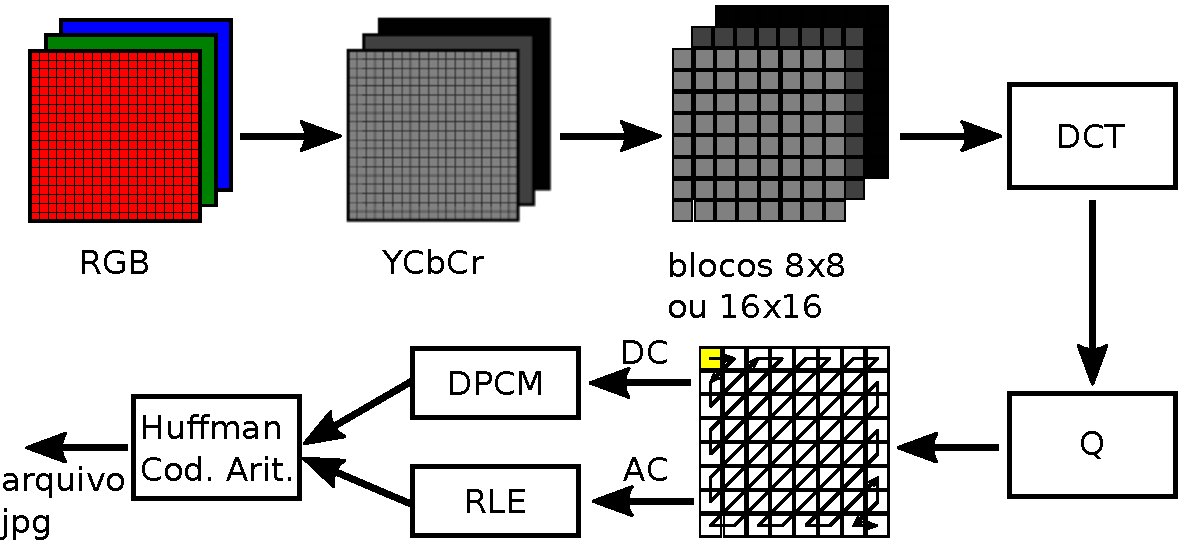
\includegraphics[width=0.8\textwidth]{images/jpegstd.pdf}
  \caption{Esquema de compressão JPEG.}\label{fig-jpegstd}
  \end{figure}
\end{frame} 

\begin{frame}%[allowframebreaks]
  \frametitle{Slides- introdução ao GNU Octave}
  \centering
  
\includegraphics[width=0.4\textwidth]{images/qrcode-octave-intro.pdf}

  \url{https://drive.google.com/open?id=1ew5fl9v_OIybsy3KdEgIvohLTcuwuru_}
\end{frame} 

\begin{frame}%[allowframebreaks]
  \frametitle{Notebook - introdução}
  \centering
  
\includegraphics[width=0.4\textwidth]{images/qrcode-jupyter-intro.pdf}

  \url{https://nbviewer.jupyter.org/github/leolca/notebooks/blob/master/aev/introducao.ipynb}
\end{frame} 

\begin{frame}%[allowframebreaks]
  \frametitle{Notebook - imagem colorida}
  \centering
  
\includegraphics[width=0.4\textwidth]{images/qrcode-jupyter-im-color.pdf}

  \url{https://nbviewer.jupyter.org/github/leolca/notebooks/blob/master/aev/introdocao_imagem_colorida.ipynb}
\end{frame} 



\section{Tecnicas Básicas de Compressão}

\begin{frame}%[allowframebreaks]
  \frametitle{Leitura}
  \centering
  
\includegraphics[width=0.4\textwidth]{images/qrcode-book-salomon.pdf}

  David Salomon, Giovanni Motta - \textit{Handbook of Data Compression}, 2010 \\ 
  \url{https://books.google.com.br/books?id=LHCY4VbiFqAC}\\
  Introduction, Basic Techniques \citep{salomon2010}
\end{frame} 

\subsection{RLE}
\begin{frame}%[allowframebreaks]
  \frametitle{Compressão RLE}
   
  Exemplo:

  string: `2. all is too well'

  codificação: `2. a@2l is t@2o we@2l'

  \vspace{1cm}
  Método MNP5 era utilizado nos modems antigos.

\end{frame}
\note{
MNP : Microcom Networking Protocol

"The MNP5 method is a two-stage process that starts with run-length encoding, followed by adaptive frequency encoding."
\citep{salomon2000}

"With MNP 5, the data received from the computer are first compressed with a simple algorithm, and then passed into the MNP 4 packetizing system for transmission. On best-case data the system offered about 2:1 compression, but in general terms about 1.6:1 was typical, at least on text. As a result a 2400 bit/s modem would appear to transfer text at ~4000 bit/s, even though the modem was still running at the same 600 baud * 4 bits per symbol rate.

This dramatic increase in throughput allowed Microcom modems to remain somewhat competitive with models from other companies that were otherwise nominally much faster. For instance, Microcom generally produced 1200 and 2400 bit/s modems using commodity parts, while companies like USRobotics and Telebit offered models with speeds up to 19200 bit/s."
(\url{https://en.wikipedia.org/wiki/Microcom_Networking_Protocol})
}


\begin{frame}%[allowframebreaks]
  \frametitle{Compressão RLE}
 
  Exemplo: uma imagem em tons de cinza com 8-bit de profundidade começa com os seguintes valores

  12, 12, 12, 12, 12, 12, 12, 12, 12, 35, 76, 112, 67, 87, 87, 87, 5, 5, 5, 5, 5, 5, 1, ...

  será comprimida como  \framebox{9},12,35,76,112,67,\framebox{3},87,\framebox{6},5,1, ...

  \vspace{1cm}
  Se utilizarmos como \textit{flag} o valor 255, então a sequência acima será expressa por

  255, 9, 12, 35, 76, 112, 67, 255, 3, 87, 255, 6, 5, 1, ...

  \vspace{1cm}
  grupos de 8

  \framebox{10000010},9,12,35,76,112,67,3,87,\framebox{100...},6,5,1, ...

\end{frame} 

\begin{frame}%[allowframebreaks]
  \frametitle{Exemplo RLE - GNU Octave}
  \centering
  
\includegraphics[width=0.4\textwidth]{images/qrcode-jupyter-rle.pdf}

  \url{https://nbviewer.jupyter.org/github/leolca/notebooks/blob/master/aev/rle_mario.ipynb}
\end{frame} 


\begin{frame}%[allowframebreaks]
  \frametitle{Move-to-Front Coding}
  Consideramos o alfabeto de símbolos $\mathcal{A}$ como uma lista 
  onde os símbolos mais frequentes estarão dispostos no início da lista.

  O método é localmente adaptativo, já que ele se adapta à frequência dos
  símbolos em cada região do fluxo de dados.
\end{frame} 


\begin{frame}%[allowframebreaks]
  \frametitle{Move-to-Front Coding - Exemplo \citep{salomon2010}}

   Exemplo:
   entrada a ser codificada: \textbf{abcddcbamnopponm}

  \begin{columns}[c]
  \column{.4\textwidth}
  C = (0, 1, 2, 3, 0, 1, 2, 3, 4, 5, 6, 7, 0, 1, 2, 3) \\
  -- utilizando move-to-front\\
  \vspace{1cm}
  C' = (0, 1, 2, 3, 3, 2, 1, 0, 4, 5, 6, 7, 7, 6, 5, 4) \\
  -- sem utilizar move-to-front 
  \column{.6\textwidth}
     \vspace{-0.2cm}
     \begin{figure}[h!]
     \centering
     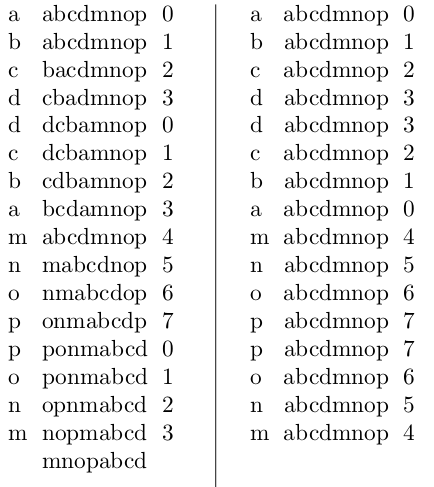
\includegraphics[width=0.7\textwidth]{images/move_to_front_coding.png}
     %\caption{}
     \label{fig:move_to_front_coding}
     \end{figure}
  \end{columns}

\end{frame} 

\begin{frame}%[allowframebreaks]
  \frametitle{Move-to-Front Coding - Exemplo \citep{salomon2010}}
  \begin{columns}[c]
  \column{.4\textwidth}
  O resultado $C$ obtido pelo move-to-front é tal que, na média, os valores
  em $C$ são pequenos (os valores no início do dicionário são os mais prováveis).
  Isto faz com que a saída seja propícia para ser codificada através da codificação
  de Huffman ou codificação aritmética.
  \column{.4\textwidth}
     \begin{figure}[h!]
     \centering
     \includegraphics[width=0.65\textwidth]{/home/leoca/ee/ufsj/2012_01/audio_video/aulas/images/variable_sized_codes.png}
     \caption{Exemplo de código de tamanho variável.}
     \label{fig:variable_sized_codes}
     \end{figure}
  \end{columns}

\end{frame}


\begin{frame}%[allowframebreaks]
  \frametitle{Move-to-Front Coding}
  Variações:
  \begin{enumerate}
  \item Move-ahead-k: O elemento do alfabeto A que corresponde ao símbolo corrente será deslocado k posições para cima na lista ao
          invés de ir para o topo da lista.
  \item Wait-c-and-move: O elemento do alfabeto A será deslocado para o início da lista apenas após aparecer c vezes durante a
          codificação. 
  item Wait-c-and-ahead-k: Um combinação das duas variantes anteriores.
  \end{enumerate}

\end{frame} 

\begin{frame}%[allowframebreaks]
  \frametitle{Exemplo Move-to-Front - GNU Octave}
  \centering
  
\includegraphics[width=0.4\textwidth]{images/qrcode-jupyter-m2f.pdf}

  \url{https://nbviewer.jupyter.org/github/leolca/notebooks/blob/master/aev/move-to-front.ipynb}
\end{frame} 





% quantização escalar
\section{Quantização Escalar}
\subsection{Conversão AD/DA}
\begin{frame}%[allowframebreaks]
  \frametitle{Conversão AD/DA}

  \begin{figure}[h]
  \centering
  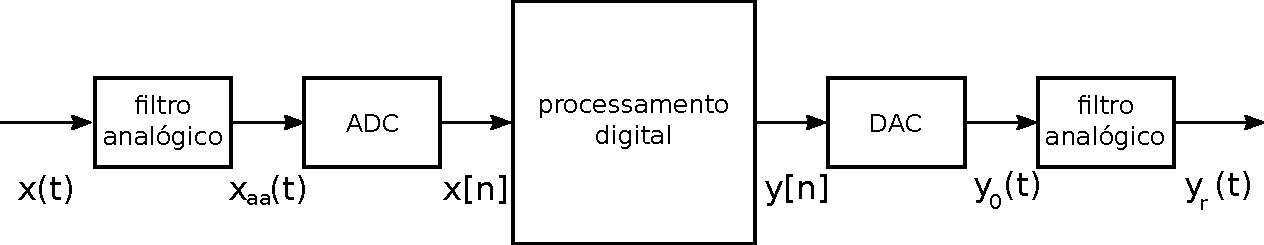
\includegraphics[width=0.7\textwidth]{images/conversaoadda.pdf}
  \caption{Processamento digital de sinais. Conversão AD e DA.}\label{fig-conv-adda}
  \end{figure}

\end{frame}


\begin{frame}%[allowframebreaks]
  \frametitle{Quantização}

  \begin{figure}[h]
  \centering
  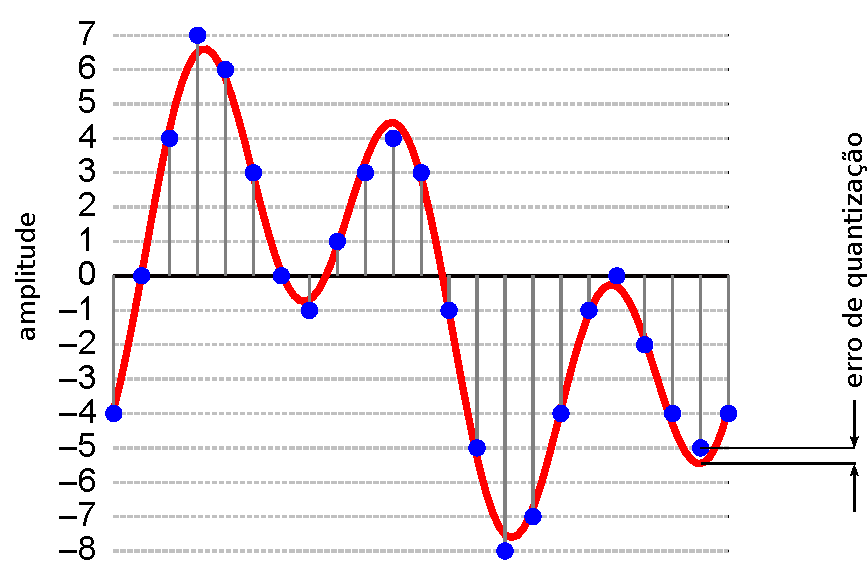
\includegraphics[width=0.5\textwidth]{images/digitalization.pdf}
  \caption{Quantização.}\label{fig-sig-quantz}
  \end{figure}

\end{frame}

\begin{frame}%[allowframebreaks]
  \frametitle{Amostragem}
  Ao amostrar um sinal $x(t)$ com período de amostragem $T_s$ teremos
  \begin{eqnarray}
  x_s(t) &=& x(t) s(t) \nonumber \\ 
        &=& x(t) \sum_{k=-\infty}^{\infty} \delta(t - kT_s) \nonumber \\
         &=& \sum_{k=-\infty}^{\infty} x(kT_s) \delta(t - kT_s)
  \end{eqnarray}

\end{frame}


\begin{frame}%[allowframebreaks]
  \frametitle{Amostragem}

  \begin{figure}[h]
  \centering
  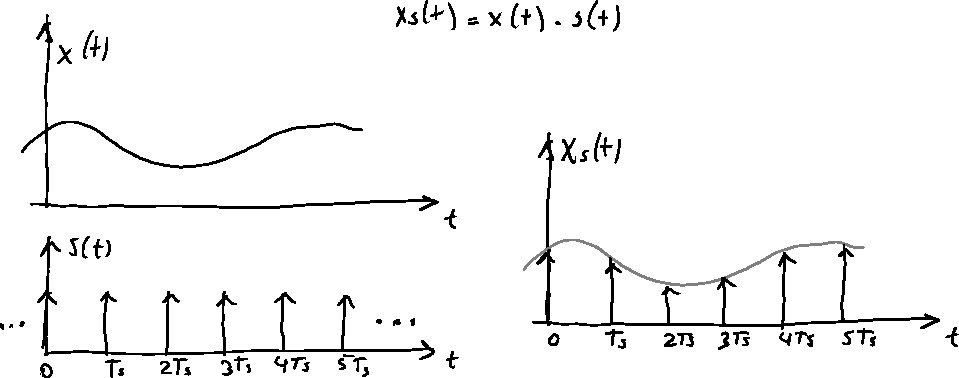
\includegraphics[width=0.8\textwidth]{images/amostragem.pdf}
  %\caption{.}
  \label{fig-amostragem}
  \end{figure}

\end{frame}

\begin{frame}[allowframebreaks]
  \frametitle{Amostragem}
  Como $s(t) = \sum_{k=-\infty}^{\infty} \delta(t - kT_s)$ é periódico com período $T_s$,
  podemos representá-lo por uma série de Fourier:
  \begin{equation}
  s(t) = \sum_{k=\infty}^{\infty} \delta(t - kT_s) = \sum_{k=-\infty}^{\infty} c_k e^{j 2 \pi t k /T_s} \textmd{,}
  \end{equation}
  onde
  \begin{equation}
  c_k = \frac{1}{T_s} \int_{-T_s/2}^{T_s/2} \delta(t) e^{-j2\pi t k/T_s} dt = \frac{1}{T_s}
  \end{equation}
  Desta forma, $x_s(t) = x(t) \cdot s(t)$ poderá ser expresso por
  \begin{equation}
  x_s(t) = \frac{1}{T_s} \sum_{k=-\infty}^{\infty} x(t) e^{j2\pi tk /T_s} \textmd{.}
  \end{equation}

  A multiplicação por $\exp(j 2\pi \alpha t)$ corresponde, na frequência, a um deslocamento de $\alpha$. 
  Teremos assim
  \begin{equation}\label{eq-Xs-freqdom}
  X_s(j \Omega) = \frac{1}{T_s} \sum_{k=-\infty}^{\infty} X \left( j (\Omega - n \Omega_s) \right)
  \end{equation}

  
  \framebreak

  Podemos chegar ao mesmo resultado sabendo que, se no domínio do tempo temos $x_s(t) = x(t) \cdot s(t)$, 
  no domínio da frequência temos
  \begin{equation}\label{eq-conv-dom-freq}
  X_s(j \Omega) = \frac{1}{2\pi} X(j \Omega) \ast S(j \Omega) .
  \end{equation} 
  Como a transformada de Fourier de $s(t)$ é
  \begin{equation}\label{eq-pulse-train-freq}
  S(j \Omega) = \frac{2\pi}{T_s} \sum_{k=-\infty}^{\infty} \delta(\Omega - k \Omega_s) ,
  \end{equation}
  onde $\Omega_s = \nicefrac{2\pi}{T}$, então utilizando as \Cref{eq-conv-dom-freq,eq-pulse-train-freq} obtemos \Cref{eq-Xs-freqdom}.

  \framebreak

  Se $x(t)$ for um sinal limitado em frequência ($\Omega_N$ frequência máxima) e
  não havendo \textit{aliasing}, $\Omega_s > 2 \Omega_N$, podemos reconstruir $x(t)$:
  \begin{equation}\label{eq-x-reconstruido}
  X_r(j \Omega) = H_r(j \Omega) X_s(j \Omega)
  \end{equation}
  onde $H_r$ é um filtro passa-baixas ideal com $\Omega_N < \Omega_c < \Omega_s$.

  \begin{equation}
  H_r (j \Omega) = \begin{cases}1 \quad & \textmd{, se \ \ } \vert \Omega \vert \leq \Omega_c,\\ 0 & \mbox{, caso contrário.}\end{cases}
  \end{equation}

  \vspace{2ex}
  (Teorema da Amostragem)

  \vspace{3ex}
  Leitura: Capítulo 4 \bibentry{oppenheim2009}.
\end{frame}



\begin{frame}%[allowframebreaks]
  \frametitle{Amostragem}

  \begin{figure}[h]
  \centering
  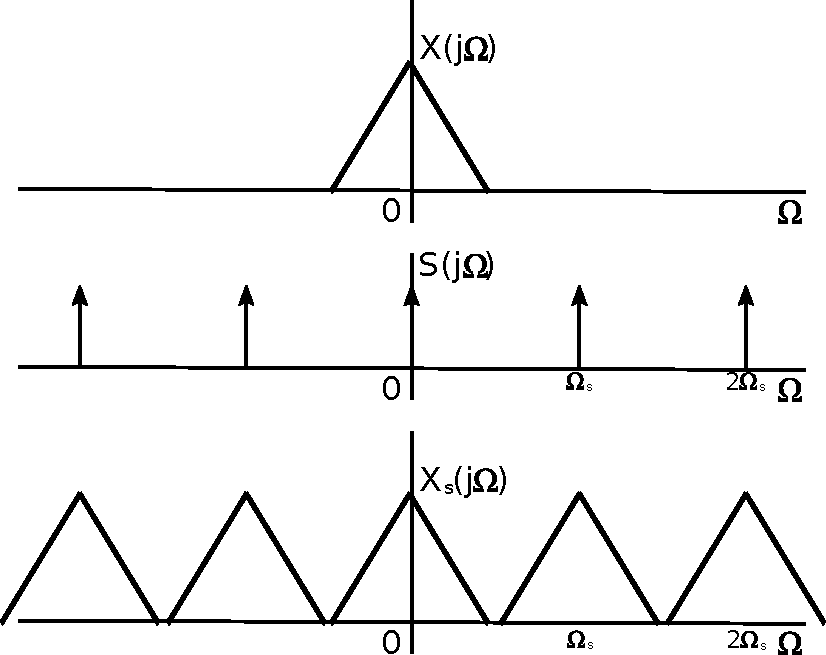
\includegraphics[width=0.6\textwidth]{images/sampling-freq-a.pdf}
  %\caption{.}
  \label{fig-sampling-freq-a}
  \end{figure}

\end{frame}

\begin{frame}%[allowframebreaks]
  \frametitle{Amostragem}

  \begin{figure}[h]
  \centering
  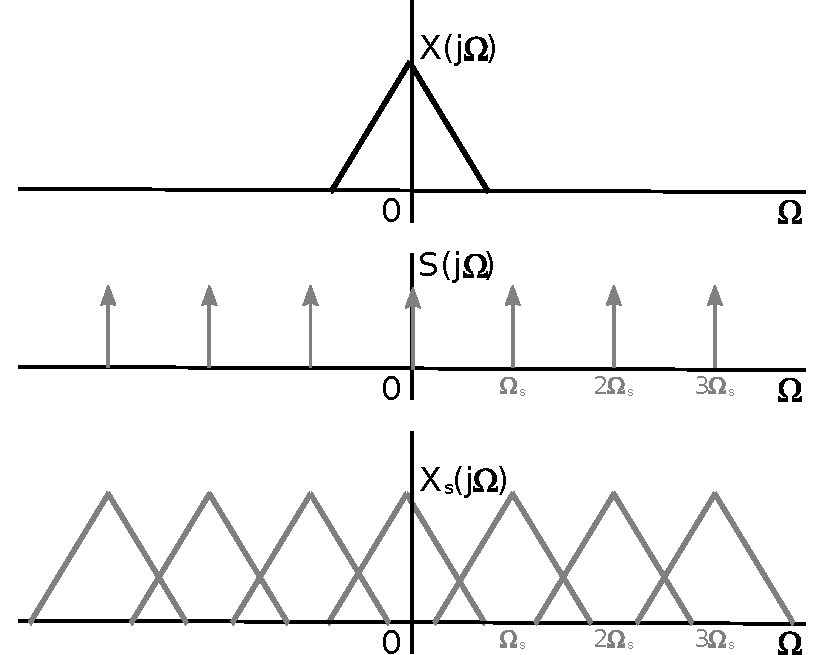
\includegraphics[width=0.6\textwidth]{images/sampling-freq-b.pdf}
  %\caption{.}
  \label{fig-sampling-freq-a}
  \end{figure}

\end{frame}


\subsection{Quantização Escalar}
\begin{frame}[allowframebreaks]
  \frametitle{Quantização Escalar}

  Quantização escalar é um mapeamento $Q$ de valores reais $x$ de uma variável aleatória
  contínua $X$ nos valores $y = Q(x)$, mais próximos de $x$ (em termos de uma determinada medida de distorção),
  de um conjunto discreto e finito $Y = {y_1 , y_2 , \ldots,  y_M }$.
  Os valores $y_i$ , $i = 1, 2, \ldots , M$, são chamados níveis de saída, ou valores de representação,
  ou ainda valores de aproximação. $Y$ é chamado de \textit{codebook} ou conjunto de aproximação.

  \framebreak

  O quantizador escalar é determinado pelo conjunto de limiares 
  $\mathcal{T} = \{t_i\}$, $i=0, 1, \ldots, M$
  e pelo conjunto de pontos de representação $\mathcal{Y} = \{y_i\}$, $i=1, \ldots, M$. 
  Os limiares dividem exaustivamente o domínio $\mathit{R}$ em subintervalos 
  (ou células, regiões de representação) $\Delta_i = (t_{i-1} , t_i ]$ disjuntas,
  ou seja, $\Delta_i \cap \Delta_j = \emptyset$. Diz-se que a divisão é exaustiva
  pois $\bigcup_{i=1}^M \Delta_i = \mathit{R}$. Esta divisão é tal que existe apenas
  um $y_i$ associado a cada intervalo $\Delta_i$, ou seja, $y_i = Q(x)$ se e somente se
  $x \in \Delta_i$. 

  \framebreak 

  \begin{figure}[h!]
  \centering
  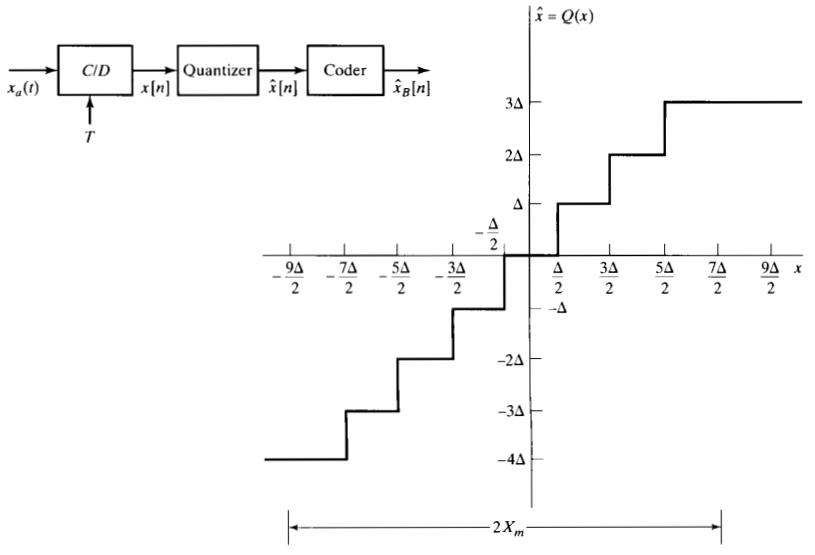
\includegraphics[width=0.6\textwidth]{images/quantization-oppenheim-fig447.png}
  \caption{Quantização. Fonte: \cite{oppenheim2009}.}
  \label{fig:quantization-fig447}
  \end{figure}  

  \framebreak

  É inerente ao processo de quantização a introdução de um erro, chamado \textit{erro de quantização}
  ou \textit{ruído de quantização}.

  O erro de quantização esperado é dado por
  \begin{equation}
  D(Q) = E\left\lbrace d(x,Q(x)) \right\rbrace ,
  \end{equation}
  onde $d(x,Q(x))$ é uma medida de distorção entre $x$ e $Q(x)$, dada por $d(\cdot)$.

  A taxa de quantização é o número de bits $R$ que é utilizado na representação de um valor $x$.
  Ela é dada em bits por amostra.

  Para um quantizador com taxa fixa temos $R = \log_2 M$ bits por amostra.

  \framebreak

  \begin{figure}[h!]
  \centering
  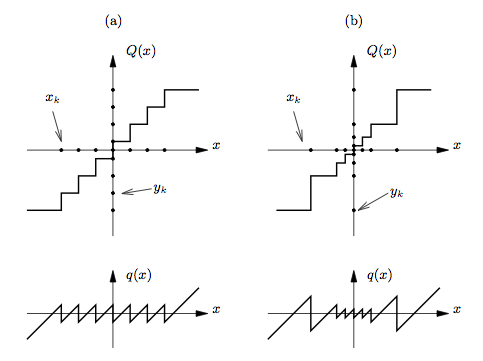
\includegraphics[width=0.55\textwidth]{/home/leoca/ee/ufsj/2012_01/audio_video/aulas/images/quantizationerror.png}
  \caption{(a) linear (b) logarítmico. Fonte: \cite{oppenheim2009}.}
  \label{fig:quantizationerror}
  \end{figure}  

\end{frame}

\subsection{Entropia na saída do quantizador}
\begin{frame}[allowframebreaks]
  \frametitle{Entropia na saída do quantizador}
  As probabilidades dos níveis de representação de um quantizador podem ser determinadas,
  conhecendo-se a pdf do sinal.

  Seja $f(x)$ a pdf (função densidade de probabilidade) de $X$. Podemos calcular a probabilidade
  do i-ésimo nível de reprodução (a probabilidade de $x \in \Delta_i$) como
  \begin{equation}
  P(y_i) = \int_{t_i -1}^{t_i} f(x) \mathrm{d}x .
  \end{equation}
  A entropia da saída do quantizador é igual a
  \begin{equation}
  H(Y) = - \sum_{i=1}^{M} P(y_i) \log_2 P(y_i) .
  \end{equation}

  Um código de comprimento variável poder ser utilizado para representar a saída 
  do quantizador (exemplo: código de Shannon, código Huffman, ou codificação aritmética).
\end{frame}
\note{
Shannon: o limite de representação é a entropia.

O limite para se representar um sinal, sem perdas, será dado pela entropia da fonte.
}


\subsection{Quantização Escalar Uniforme}
\begin{frame}[allowframebreaks]
   \frametitle{Quantização escalar uniforme}
  A quantização escalar é uniforme quando os limiares estão igualmente espaçados,
  e desta forma, as células possuem o mesmo tamanho (exceto as extremas, primeira e última),
  ou seja, $\vert \Delta_i \vert = \delta$, e o ponto de representação localiza-se no 
  ponto médio da célula,
  \begin{equation}
  y_i = \frac{t_{i-1} + t_i}{2} = t_{i-1} + \frac{\delta}{2} , \ \ i=1,2,\ldots,M .
  \end{equation}

  \framebreak

  (*obs.: considerando apenas valores positivos)

  Dada a entrada $x$, a célula associada a $x$ é determinada por
  \begin{equation}
  i = [x / \delta ] ,
  \end{equation}
  onde $\delta$ é a largura de cada célula e $[ \cdot ]$ representa a operação
  de arredondamento.
 
  O valor de aproximação para a entrada $x$ é dado por
  \begin{equation}
  y = Q(x) = \delta \left[ \frac{x}{\delta} \right]   
  \end{equation}
  isto é, a i-ésima célula é determinada por $\Delta_i = (i\delta - \delta/2, i\delta + \delta/2]$
  e $y_i = i\delta$.

\end{frame}

\begin{frame}%[allowframebreaks]
   \frametitle{Distorção no quantizador escalar uniforme}
  Se $f(x)$ é conhecida, então podemos calcular a distorção esperada do quantizador
  \begin{equation}
  D(Q) = \int_{-\infty}^{\infty} f(x) d(x,Q(x)) dx = \sum_i \int_{t_{i-1}}^{t_i} f(x) d(x,y_i) \mathrm{d}x .
  \end{equation}

  Se o erro de distorção é medido pelo erro quadrático, então $D(Q)$ fornecerá o 
  erro quadrático médio (MSE, \textit{Mean Squared Error}):
  \begin{equation}
  D(Q) = \sum_i \int_{t_{i-1}}^{t_i} f(x) (x - y_i)^2 \mathrm{d}x .
  \end{equation}
\end{frame}




\subsection{Quantização Escalar Não-Uniforme}

\begin{frame}[allowframebreaks]
   \frametitle{Quantização escalar não-uniforme}
 
  Se conhecemos as características estatísticas de $X$, podemos utilizar esta informação
  para melhorar as características do quantizador.

  \begin{figure}[h!]
  \centering
  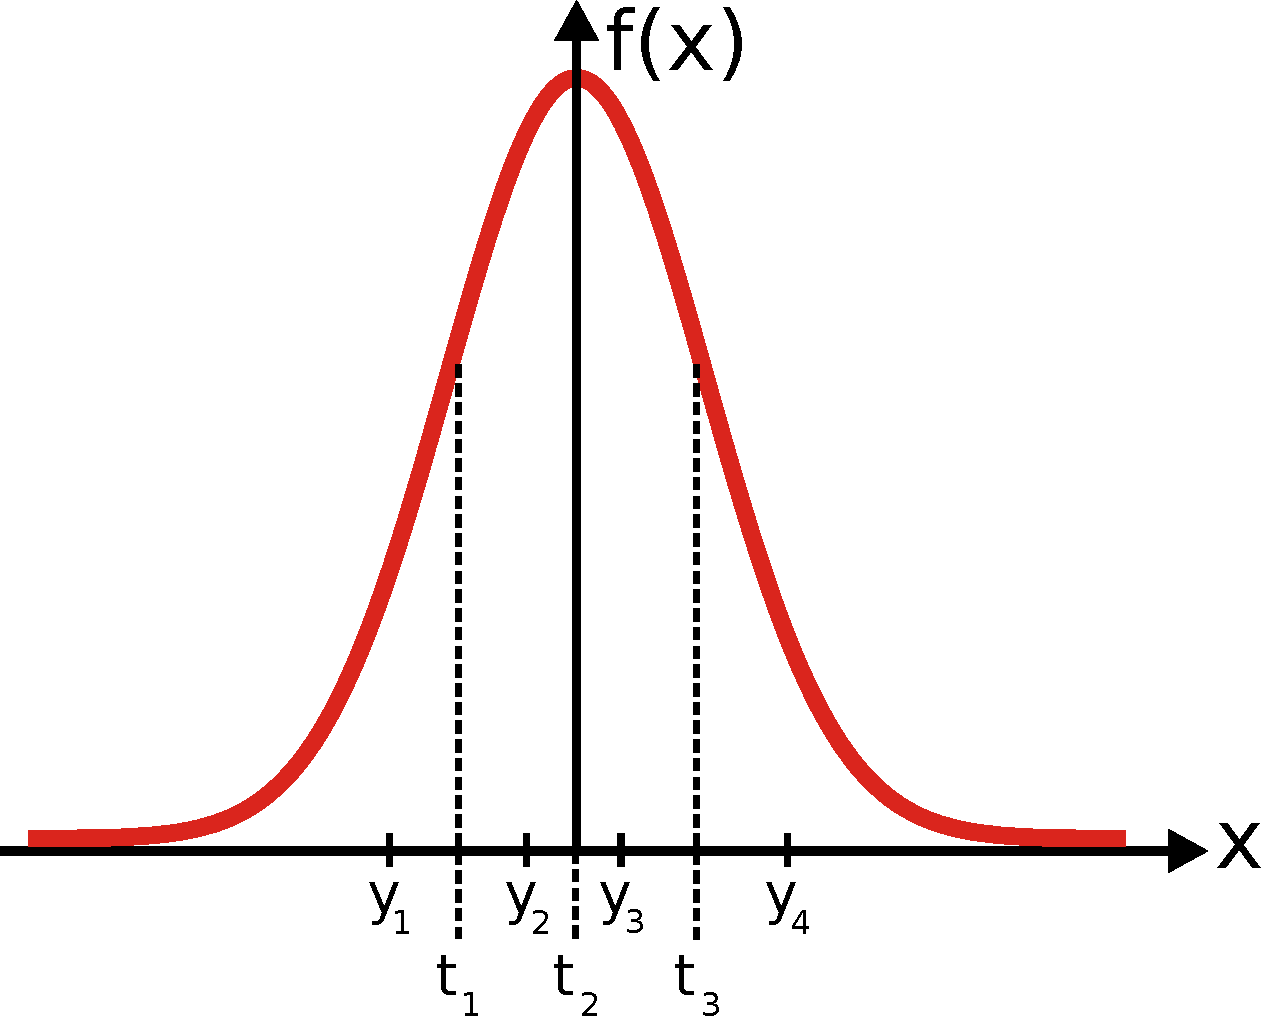
\includegraphics[width=0.45\textwidth]{images/quantz-gaussian.pdf}
  %\caption{}
  \label{fig:quantz-gaussian}
  \end{figure}  
\end{frame}



\subsection{Lloyd-Max}
\begin{frame}[allowframebreaks]
  \frametitle{Algoritmo de Lloyd-Max}
  O algoritmo de \emph{Lloyd-Max} é um algoritmo para encontrar os limiares $\{t_i\}$ e
  os pontos de representação $\{y_i\}$ que minimizam a distorção.

  Lloyd e Max criaram um procedimento para construir uma solução para o problema, que satisfaz
  as condições necessárias (mas não suficientes):

  \begin{itemize}
  \item os limiares devem ficar entre os pontos de representação:
        \begin{equation}
        t_i = \frac{y_{i+1} + y_{i}}{2} \quad , 1 \leq i \leq M-1 , 
        \end{equation}
  \item os pontos de representação devem ficar no meio (com relação à esperança) de um dado intervalo
        \begin{equation}
        y_i = E [ X(i) ] = \frac{ \int_{t_{i-1}}^{t_i} x f_X (x) dx }{ \int_{t_{i-1}}^{t_i} f_X (x) dx  } .
        \end{equation}
  \end{itemize}

  \framebreak
  Algoritmo:
  \begin{enumerate}
  \item Escolher um conjunto inicial arbitrário com $M$ pontos de representação $y_1 < y_2 < \ldots y_M$.
  \item Para cada $i$, $1 \leq j \leq M-1$, fazer $t_i = \frac{1}{2} (y_{i+1} + y_i)$.
  \item Para cada $i$, $1 \leq j \leq M-1$, fazer $y_i$ igual à média condicional de $X \sim f(x)$,
        dado $X \in (t_{i-1}, t_i]$ (onde $t_0$ e $t_M$ são respectivamente $-\infty$ e $+\infty$).
  \item Repetir os passos (2) e (3) até que a melhoria no MSE seja desprezível; então interromper.
  \end{enumerate}
  O MSE decresce (ou permanece o mesmo) a cada passo do algoritmo. Como o MSE é não-negativo,
  ele irá se aproximar de um limite em um número finito de passos, pois o algoritmo será interrompido
  quando a melhoria no MSE foi menor que um dado $\epsilon > 0$.

  \framebreak
  O exemplo abaixo ilustra que o algoritmo deve chegar a um mínimo local.
  Considere $M=2$ pontos de representação e uma pdf $f(x)$ como definida na Figura \ref{fig:lloyd-ex}.

  \begin{figure}[h!]
  \centering
  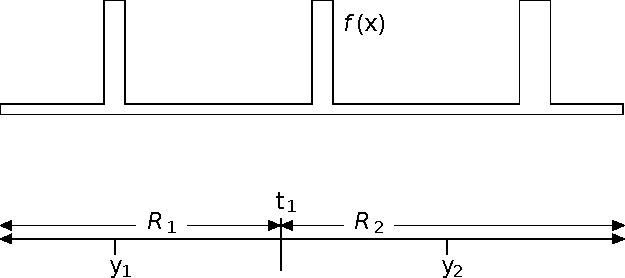
\includegraphics[width=0.55\textwidth]{images/lloyd-ex.pdf}
  \caption{Exemplo Lloyd-Max: regiões e pontos de representação que satisfazem 
        a condição de parada do algoritmo nas não minimizam a distorção média quadrática.
	Fonte: \citet{gallager2008}}
  \label{fig:lloyd-ex}
  \end{figure}

  \framebreak

  A configuração apresentada na Figura \ref{fig:lloyd-ex} satisfaz os critérios de parada, entretanto
  o pico mais a direita é mais provável que os outros dois, desta forma, o MSE poderia ser menor se 
  $R_1$ cobrisse a regiões dos dois picos à esquerda e $R_2$ apenas o pico à direita.

  \vspace{2ex}
  Leitura: Capítulo 3 \bibentry{gallager2008}.
\end{frame}







\subsection{Performance do Quantizador}

\begin{frame}[allowframebreaks]
  \frametitle{Performance do Quantizador}
  Seja $p(x)$ a pdf do sinal de entrada $x$, então o erro médio quadrático (MSE) 
  devido à quantização será dado por
  \begin{equation} \label{eq-sqnr-quants}
  \sigma_q^2 = \sum_{k=1}^{M} \int_{t_{k-1}}^{t_k} (x - y_k)^2 p(x) \mathrm{d}x.
  \end{equation}

  Se $M$ for grande e a pdf $p(x)$ for suave, poderemos aproximar $p(x)$ no intervalo $(t_{k-1},t_{k}]$ como
  \begin{equation}
  p(x) \approx p\left(\frac{t_{k-1}+t_{k}}{2}\right) , \quad t_{k-1} < x \leq t_k ,
  \end{equation}
  e assim, a equação \ref{eq-sqnr-quants} poderá ser reescrita como
  \begin{equation} \label{eq-sqnr-quants2}
  \sigma_q^2 = \sum_{k=1}^{M} p\left(\frac{t_{k-1}+t_{k}}{2}\right) \int_{t_{k-1}}^{t_k} (x - y_k)^2 \mathrm{d}x.
  \end{equation}

  Mostra-se que
  \begin{equation} \label{eq-sqnr-int}
  \int_{t_{k-1}}^{t_k} (x - y_k)^2 \mathrm{d}x = \Delta_k \left[ \left( y_k - \frac{t_{k-1} + t_{k}}{2} \right)^2 + \frac{\Delta_k^2}{12} \right] ,
  \end{equation}
  onde $\Delta_k = t_k - t_{k-1}$ é o tamanho do passo do quantizador.

  Para minimizar o MSE devemos escolher $y_k = (t_{k-1} + t_{k})/2$, 
  de forma que o primeiro termo em \ref{eq-sqnr-int} se anule. Ou seja,
  devemos escolher os pontos de representação como o ponto médio dos limiares dos intervalos.
  (obs.: Isto ocorre devido à aproximação feita para $p$ suave e $M$ grande. No caso geral,
  deveremos ter os pontos de representação no valor esperado de cada intervalo)

  Vamos definir $p_k$ como a probabilidade de $x$ pertencer ao intervalo $(t_{k-1},t_k]$.
  Usando a aproximação feita anteriormente, teremos
  \begin{equation} \label{eq-pk-aprox}
  p_k = \Pr(t_{k-1} < x \leq t_k) \approx p\left(\frac{t_{k-1}+t_{k}}{2}\right) \Delta_k ,
  \end{equation}
  e assim podemos reescrever a equação \ref{eq-sqnr-quants2} como
  \begin{equation} \label{eq-sqnr-quants3}
  \sigma_q^2 = \frac{1}{12} \sum_{k=1}^{M} p_k \Delta_k^2 .
  \end{equation}

\end{frame}


\subsection{Quantizador Uniforme}
\begin{frame}[allowframebreaks]
  \frametitle{Performance do Quantizador Uniforme} 

  Para o quantizador uniforme o passo é constante ($\Delta_k = \Delta$ para todo $k$). Teremos assim
  \begin{equation} \label{eq-sqnr-quants-uni}
  \sigma_q^2 = \frac{\Delta^2}{12} \underbrace{ \sum_{k=1}^{M} p_k }_{=1} = \frac{\Delta^2}{12} .
  \end{equation}
  Note que a potência do ruído de quantização é independente da distribuição do sinal.

  A performance do quantizador será expressa pela relação sinal-ruído de quantização (SQNR),
  \begin{equation} \label{eq-sqnr-unif}
  \textmd{SQNR} = 10 \log \left( \frac{\sigma_x^2}{\sigma_q^2} \right) = 10 \log \left( \frac{12 \sigma_x^2}{\Delta^2} \right) \mathrm{dB}.
  \end{equation}
\end{frame}

\begin{frame}[allowframebreaks]
  \frametitle{Performance do Quantizador Uniforme - Sinal Senoidal}
  Vamos supor que o sinal de entrada seja da forma $A \sin \omega t$ e 
  um quantizador uniforme com $n$ bits ($2^n = M$). Podemos escolher $\Delta$
  para que não ocorra saturação. Faremos então $\Delta = A/2^{n-1}$.
  A potência do sinal senoidal é $\sigma_x^2 = A^2/2$. Usando agora a Equação \ref{eq-sqnr-unif}, teremos
  \begin{equation} \label{eq-sqnr-unif-sin}
  \textmd{SQNR (senoide)}  = 6n + 1.76 \mathrm{dB}.
  \end{equation}
\end{frame}

\begin{frame}[allowframebreaks]
  \frametitle{Performance do Quantizador Uniforme - Sinal Gaussiano}
  Iremos supor agora um sinal de entrada com distribuição gaussiana: $p(x)=1/\sqrt{2\pi\sigma} e^{-(x^2/2\sigma^2)}$.
  Para que a distorção por saturação seja desprezível, iremos fazer $2^{n-1} \Delta = 4 \sigma$, ou seja, teremos $\Delta = \sigma/2^{n-3}$.
  A potência média quadrática do sinal de entrada é $\sigma_x^2 = \sigma^2$. Usando agora a Equação \ref{eq-sqnr-unif}, teremos
  \begin{equation} \label{eq-sqnr-unif-gaus}
  \textmd{SQNR (gauss)}  = 6n - 7.3 \mathrm{dB}.
  \end{equation}
\end{frame}


\subsection{Quantizador Não Uniforme}
\begin{frame}%[allowframebreaks]
  \frametitle{Quantizador Não Uniforme}

  Os sinais de fala, por exemplo, estão geralmente concentrados em torno da origem.
  Desta forma, seria interessante propor um quantizador em que os passos de quantização
  fossem menores na região de menor amplitude do sinal e maiores na região de maior amplitude.
  Isto levaria a uma redução do ruído de quantização total.

  \begin{figure}[h!]
  \centering
  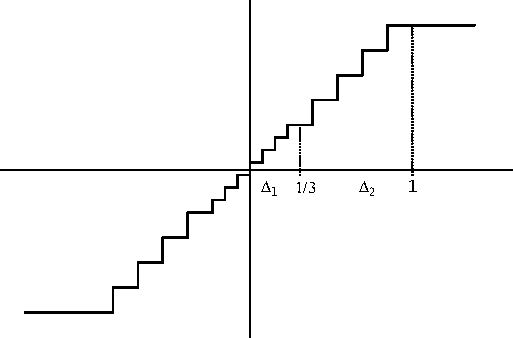
\includegraphics[width=0.4\textwidth]{images/nuquantz.pdf}
  \caption{Exemplo de quantizador não uniforme de 4 bits, com $\Delta_1 = \Delta_2/2$ \citep{tokunbo}.}
  \label{fig:nuquantz}
  \end{figure}
\end{frame}


\subsection{Compressor e Expansor}
\begin{frame}%[allowframebreaks]
  \frametitle{Compressor e Expansor}
  Podemos utilizar compressor e expansor para implementar um quantizador não uniforme.

  \begin{description}
  \item[compressor] é feito para amplificar os sinais de baixa amplitude, às custas de atenuar os sinais de alta amplitude;
  \item[expansor] faz o inverso.
  \end{description}

  \begin{figure}[h!]
  \centering
  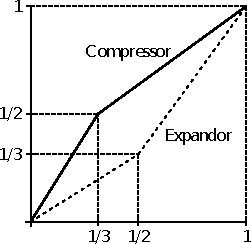
\includegraphics[width=0.3\textwidth]{images/compressor.pdf}
  \caption{Exemplo de compressor e expansor \citep{tokunbo}.}
  \label{fig:compressor}
  \end{figure}
\end{frame}


\begin{frame}[allowframebreaks]
  \frametitle{Performance do Quantizador Não Uniforme}

  O erro médio quadrático devido à quantização é dado pela Equação \ref{eq-sqnr-quants3}, repetida a seguir,
  \begin{equation} 
  \sigma_q^2 = \frac{1}{12} \sum_{k=1}^{M} p_k \Delta_k^2  , \nonumber
  \end{equation}
  onde $p_k = \Pr(t_{k-1} < x \leq t_k)$ e $\Delta_k = (t_k - t_{k-1})$.

  Suponha que o compressor apresentado na Figura \ref{fig:excompressor} seja utilizado.
  \begin{figure}[h!]
  \centering
  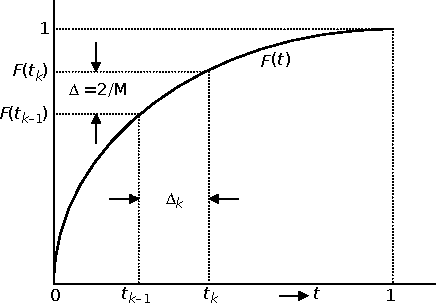
\includegraphics[width=0.6\textwidth]{images/excompressor.pdf}
  \caption{Exemplo de compressor \citep{tokunbo}.}
  \label{fig:excompressor}
  \end{figure}

  Os limiares $t_{k-1}$ e $t_{k}$, correspondentes a um codificador não uniforme, são mapeados 
  através da função compressora $F(\cdot)$ nos limiares $F(t_{k-1})$ e $F(t_k)$, uniformemente espaçados.
  Supondo o sinal no intervalo $[-1,+1]$, teremos $\Delta = 2/M$, o passo do codificador uniforme.
  Conhecendo $\Delta$ e a derivada (inclinação) de $F(t)$ no intervalo $[t_{k-1},t_{k}]$, podemos 
  determinar $\Delta_k$,
  \begin{equation}\label{eq-dk-F}
  \Delta_k = \frac{\Delta}{F'(t_k^{\ast})} = \frac{2}{M F'(t_k^{\ast})}, \quad t_{k-1} < t_k^\ast < t_k .
  \end{equation} 

  Substituindo $\Delta_k$ na Equação \ref{eq-sqnr-quants3}, teremos
  \begin{equation} \label{eq-sqnr-q-nu}
  \sigma_q^2 = \frac{1}{3} \sum_{k=1}^{M} \frac{p_k}{M^2 (F'(t_k^{\ast}))^2} , \quad t_{k-1} < t_k^\ast < t_k .
  \end{equation}

  Se o número de níveis $M$ for grande, o somatório em \ref{eq-sqnr-q-nu} poderá ser aproximado por
  uma integral:
  \begin{equation} \label{eq-sqnr-q-nu2}
  \sigma_q^2 = \frac{1}{3M^2} \int_{-1}^{+1} \frac{p(x)}{ (F'(x))^2 } \mathrm{d}x = \frac{2}{3M^2} \int_{0}^{+1} \frac{p(x)}{ (F'(x))^2 } \mathrm{d}x  ,
  \end{equation}
  onde utilizamos a simplificação em que a $p(x)$ é simétrico par.

  Para um sinal com excursão entre $-X_m$ e $+X_m$, teremos
  \begin{equation} \label{eq-sqnr-q-nu2}
  \sigma_q^2 = \frac{2 X_m^2}{3M^2} \int_{0}^{X_m} \frac{p(x)}{ (F'(x))^2 } \mathrm{d}x  .
  \end{equation} 

\end{frame}

\begin{frame}[allowframebreaks]
  \frametitle{Compressão Logarítmica}
  Em um sistema de telecomunicações, desejamos uma SNR constante, independente da distribuição do sinal de entrada.
  Desejamos então encontrar o compressor $F$ que alcança este objetivo.

  \begin{equation} \label{eq-sqnr-log-const}
  \textmd{SNR} = \frac{\sigma_x^2}{\sigma_q^2} = \frac{2 \int_0^1 x^2 p(x) \mathrm{d}x}{ \frac{2}{3M^2} \int_0^1 \frac{p(x)}{(F'(x))^2} \mathrm{d}x } .
  \end{equation}
  A expressão em \ref{eq-sqnr-log-const} pode ser feita constante escolhendo
  \begin{equation} \label{eq-dcompr}
  F'(x) = \frac{k^{-1}}{x} ,
  \end{equation}
  com parâmetro $k$ a ser especificado.

  A curva de compressão $F(x)$ é obtida realizando-se a integração e escolhendo a constante de integração 
  para que a condição de contorno $F(1)=1$ seja satisfeita, obtendo assim
  \begin{equation} \label{eq-compr}
  F(x) = 1 + k^{-1} \ln x .
  \end{equation}
  Para este caso a SNR obtida será
  \begin{equation} \label{eq-sqnr-log-const2}
  \textmd{SNR} =  \frac{3M^2}{k^2} .
  \end{equation}
  Para sinal com extensão de $-X_m$ a $X_m$, teremos
  \begin{equation} \label{eq-compr2}
  F(x) = X_m + k^{-1} \ln \left(\frac{x}{X_m}\right) .
  \end{equation}

  \begin{figure}[h!]
  \centering
  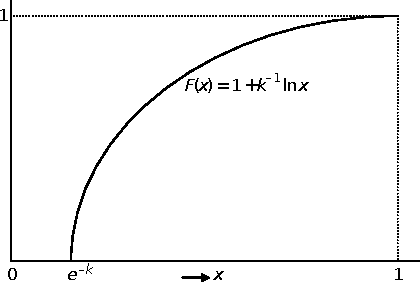
\includegraphics[width=0.6\textwidth]{images/Fx.pdf}
  \caption{Gráfico de $F(x) = 1 + k^{-1} \ln x$ \citep{tokunbo}.}
  \label{fig:Fx}
  \end{figure}

  Através da Equação \ref{eq-dk-F} e da escolha feita em \ref{eq-dcompr}, podemos verificar
  que o tamanho do passo de quantização é proporcional à amplitude do sinal, quando utilizamos
  a compressão logarítmica dada por $F(x) = 1 + k^{-1} \ln x$. 
  \begin{equation}
  \Delta_k = \frac{2}{M F'(t_k^{\ast})} = \frac{2}{M k^{-1}} t_k^{\ast} .
  \end{equation}
  Para valores próximo da origem,
  esta proporcionalidade não poderá ser mantida, pois $\ln x$ diverge
  quando $x \rightarrow 0$.

  Uma lei de compressão prática não pode ter tal descontinuidade, devendo também especificar a compressão
  dada a sinais de baixa amplitude.
\end{frame}

\begin{frame}[allowframebreaks]
  \frametitle{lei $\mu$}
   Esta aproximação desloca o cruzamento com zero de $F(x)$, 
   que ocorria em $x = e^{-k}$, para a origem.

   \begin{equation}
   F(x) = \frac{\log (1 + \mu x)}{ \log (1 + \mu)} , \quad 0 \leq x \leq 1 ,
   \end{equation}
   onde a base do logaritmo é irrelevante.

  \begin{equation}
   F(x) = \sign (x) \frac{\log (1 + \mu |x|)}{ \log (1 + \mu)} , \quad -1 \leq x \leq 1 .
  \end{equation}

  \framebreak

  Note que, quando $\mu \gg 1$, esta lei aproxima uma curva logaritma para valores grandes.
  \begin{equation}
  F(x) = \frac{\log (1 + \mu x)}{\log(1+\mu)} \approx \frac{\log(\mu x)}{\log(\mu)} = 1 + \frac{\log(x)}{\log(\mu)} = 1 + \frac{\ln x}{\ln \mu} .
  \end{equation}
  Teremos então $k = \ln \mu$ e assim a SNR para sinais grandes será aproximadamente $3M^2/(\ln \mu)^2$.

  \framebreak

  \begin{figure}[h!]
  \centering
  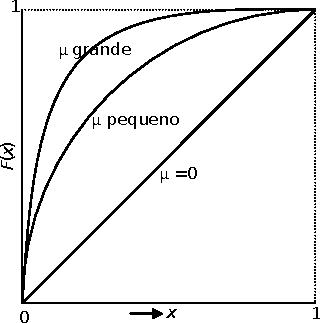
\includegraphics[width=0.4\textwidth]{images/mulaw.pdf}
  \caption{Curva de compressores segundo a lei $\mu$ \citep{tokunbo}.}
  \label{fig:mulaw}
  \end{figure}
  
  A lei $\mu$ é utilizada no padrão ITU G.711 PCM através de uma aproximação discreta usando $\mu=255$.
\end{frame}

\begin{frame}[allowframebreaks]
  \frametitle{lei A}

  \begin{figure}[h!]
  \centering
  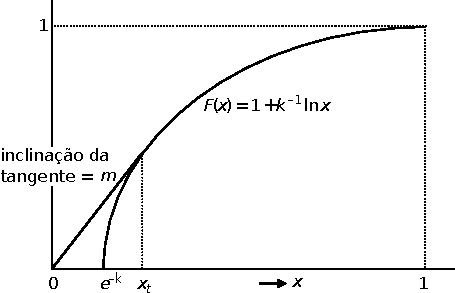
\includegraphics[width=0.6\textwidth]{images/Alaw.pdf}
  \caption{Curva de compressores segundo a lei A \citep{tokunbo}.}
  \label{fig:Alaw}
  \end{figure}

  \begin{equation}
  k = 1 + \ln A .
  \end{equation}

  \begin{equation}
  F(x) = \begin{cases}
  \frac{Ax}{1+\ln A} , \quad 0 \leq x \leq 1/A , \\
  \frac{1+\ln Ax}{1+\ln A}, \quad 1/A \leq x \leq 1 .
  \end{cases}
  \end{equation}

  \bibentry{tokunbo}
  %\printbibliography[keyword={tokunbo},title={Mais informações:}]
\end{frame}


\subsection{Quantização Vetorial}

\begin{frame}[allowframebreaks]
  \frametitle{Quantização Vetorial}
  Utilizamos a quantização vetorial em casos em que o sinal de entrada já é um sinal digital
  e queremos obter uma representação comprimida da informação origial (em geral, representando
  os dados originais através de um \textit{codebook}).

  \vspace{1cm}
  Considere uma variável aleatória $X$ que assumule valores $x \in \mathcal{X} \subseteq \mathit{R}$,
  e $\mathcal{X}^n \subseteq \mathit{R}^n$ o conjunto de vetores $\mathbf{x} = (x_1, x_2, \ldots, x_n) \in \mathit{R}^n$.

  \framebreak

  Uma quantização vetorial é um mapeamento $Q$  de vetores de entrada $\mathbf{x} = (x_1, x_2, \ldots, x_n )$,
  onde $\mathbf{x} \in \mathcal{X}^n$, nos valores $\mathbf{y} = (y_1 , y_2 , \ldots , y_n ) \in \mathcal{X}^n$
  mais próximos (com relação a alguma medida de distorção), onde $\mathbf{y} \in \mathcal{Y} \subseteq \mathcal{X}^n$,
  sendo $\mathcal{Y} = \{y_1 , y_2 , \ldots, y_M\}$, um subconjunto constituído por $M$ elementos em $\mathcal{X}^n$.
  O parâmetro $n$ indica a dimensionalidade dos dados e do quantizador. O conujunto de aproximação $\mathcal{Y}$ 
  é chamado de \textit{codebook}.

  \vspace{3em}
  Para se projetar um quantizador, devemos dividir o domínio $\mathcal{X}^n$ em $M$ áreas ou células $S_i$,
  $i = 1, 2, \ldots, M$, de forma que $\bigcup_i S_i = \mathcal{X}^n$, $S_i \cap S_j = \emptyset$, $i \neq j$,
  e $y_i \in S_i$.
\end{frame}


\begin{frame}[allowframebreaks]
  \frametitle{Erro de quantização médio}
  O erro de quantização esperado de um quantizador é dado por
  \begin{equation}
  D_n(Q) = E \{ d(\mathbf{x},Q(\mathbf{x})) \}
  \end{equation}

  Utilizando a distância Euclideana normalizada como métrica
  \begin{eqnarray}
  d(\mathbf{x},\mathbf{y}) &=& \frac{1}{n} d^2_E(\mathbf{x},\mathbf{y}) \nonumber \\
                           &=& \frac{1}{n} (\mathbf{x} - \mathbf{y}) (\mathbf{x} - \mathbf{y})^T \nonumber \\
                           &=& \frac{1}{n} \sum_{i=1}^n (x_i - y_i)^2 = \frac{1}{n} \Vert \mathbf{x} - \mathbf{y} \Vert^2
  \end{eqnarray}
  teremos
  \vspace{-1ex}
  \begin{equation}
  D_n (Q) = \frac{1}{n} E \{ \Vert \mathbf{x} - Q(\mathbf{x}) \Vert^2 \} = \frac{1}{n} \sum_{i=1}^M  E \{ \Vert \mathbf{x} - \mathbf{y_i} \Vert^2 \} .
  \label{eq:avg_quant_error}
  \end{equation}
 
  \framebreak
  Considere que a pdf n-dimensional dos dados, $f(\mathbf{x})$, sobre o conjunto $\mathcal{X}^n$ seja conhecida, 
  então a Equação \ref{eq:avg_quant_error} assume a forma 
  \begin{equation}
  D_n (Q) = \frac{1}{n} \sum_{i=1}^M \int_{S_i} f(\mathbf{x}) \Vert \mathbf{x} - \mathbf{y_i} \Vert^2 \mathrm{d}\mathbf{x} ,
  \end{equation}
  e a probabilidade do vetor de representação $\mathbf{y_i}$ é dada por
  \begin{equation}
  P(\mathbf{y_i}) = \int_{S_i} f(\mathbf{x}) \mathrm{d}\mathbf{x} .
  \end{equation}
\end{frame} 


\begin{frame}%[allowframebreaks]
  \frametitle{Taxa de quantização}
  A taxa de quantização $R$ é o número de bits necessários para representar o vetor $\mathbf{x}$
  (utilizando vetores de \textit{codebook} de tamanho $M$) por dimensão, $n$. Para um quantizador com taxa fixa
  (em que cada símbolo é codificado por palavras de mesmo tamanho em um dado \textit{codebook}), 
  a taxa é dada por
  \begin{equation}
  R = \frac{\log_2 M}{n} \textmd{ bits/amostra}.
  \end{equation}

  Para um quantizador de taxa variável, a taxa estará limitada pela entropia, ou seja,
  \begin{equation}
  R \geq - \frac{1}{n} \sum_{i=1}^M P(\mathbf{y_i}) \log_2 P(\mathbf{y_i}) \textmd{ bits/amostra}.
  \end{equation}
\end{frame}

\begin{frame}[allowframebreaks]
  \frametitle{Quantização vetorial}
  As células criadas por um quantizador vetorial em $n$-dimensões são regiões de Voronoi.

  O caso especial em que o \textit{codebook} gera uma estrutura regular é chamado 
  de quantizador vetorial em treliça (\textit{lattice vector quantizers}).

  \begin{figure}[h!]
  \centering
  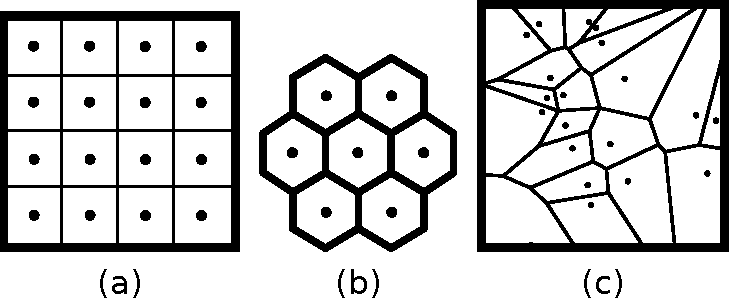
\includegraphics[width=0.6\textwidth]{images/lattice.pdf}
  \caption{Diagramas de Voronoi. Estruturas em treliça em (a) e (b).}
  \label{fig:lattice}
  \end{figure} 
\end{frame}

\begin{frame}%[allowframebreaks]
  \frametitle{Exemplo Quantização - GNU Octave}
  \centering
  
\includegraphics[width=0.4\textwidth]{images/qrcode-jupyter-quantizacao.pdf}

  \url{https://nbviewer.jupyter.org/github/leolca/notebooks/blob/master/aev/quantization.ipynb}
\end{frame} 


\begin{frame}%[allowframebreaks]
  \frametitle{Exemplos de utilização}
  A quantização vetorial é utilizada em
  \begin{itemize}
  \item Video codecs: Cinepak, Sorenson codec, Indeo, VQA (utilizada em jogos)
  \item Audio codecs: CELP, G.729, TwinVQ, Ogg Vorbis, AMR-WB+, DTS
  \end{itemize}
\end{frame}





\bibliographystyle{apalike}
\bibliography{bibliografia}
\label{bibliografia}

\end{document}

